\documentclass[11pt,titlepage]{article}
\usepackage{ucs}
\usepackage[utf8x]{inputenc}
\usepackage[T1]{fontenc}
\usepackage[ngerman]{babel}
\usepackage{graphicx}
\usepackage{titlesec}
\usepackage{url}
\usepackage{lastpage}
\usepackage{listings}
\usepackage{color}
\usepackage{fancyhdr}
\usepackage{geometry}
\usepackage{wrapfig}
\usepackage{float}
\usepackage{subcaption}
\usepackage{hyperref}
\usepackage{ragged2e}
\usepackage{framed}
\usepackage{quoting}
\usepackage{lscape}
\usepackage[table]{xcolor}
\usepackage{pdfpages}
% remove current style and use fancyplain
\pagestyle{fancyplain}
\fancyhf{}
% remove rule/lines as well
\renewcommand{\headrulewidth}{0pt}
\renewcommand{\footrulewidth}{0pt}
% set papersize, magin and footersize
\geometry{a4paper,portrait,left={3cm},right={3cm},top={2cm},bottom={1cm},includefoot,foot={1cm}}
% set footer
\rfoot{Seite \thepage \hspace{1pt} von \pageref{LastPage}}
% define some colors
\definecolor{lightgray}{rgb}{.95,.95,.95}
\definecolor{shadecolor}{rgb}{.95,.95,.95}
\definecolor{darkgray}{rgb}{.4,.4,.4}
\definecolor{purple}{rgb}{0.65, 0.12, 0.82}
% set color and font of ''\url''
\renewcommand\UrlFont{\color{blue}\rmfamily\itshape}
% colorbox which can wrap lines
\newcommand\code[1]{\codehelp#1 \relax\relax}
\def\codehelp#1 #2\relax{\allowbreak\grayspace\codecolor{#1}\ifx\relax#2\else
 \codehelp#2\relax\fi}
\newcommand\codecolor[1]{\colorbox{lightgray}{\textcolor{black}{%
  \ttfamily\mystrut\smash{\detokenize{#1}}}}}
\def\mystrut{\rule[\dimexpr-\dp\strutbox+\fboxsep]{0pt}{%
 \dimexpr\normalbaselineskip-2\fboxsep}}
\def\grayspace{\hspace{0pt minus \fboxsep}}
% add ''\code'' to highligth single code lines
%\newcommand{\code}[1]{\wrapcolorbox[lightgray]{\ttfamily{#1}}}

% add ''\shadedquotation'' to highligth quoates
\newenvironment{shadedquotation}
 {\begin{shaded*}
  \quoting[leftmargin=0pt, vskip=0pt]
 }
 {\endquoting
 \end{shaded*}
}

% define ''JavaScript'' as a language for enviroment ''lstlisting''
\lstdefinelanguage{JavaScript}{
  keywords={typeof, new, true, false, catch, function, return, null, catch, switch, var, if, in, while, do, else, case, break},
  keywordstyle=\color{blue}\bfseries,
  ndkeywords={class, export, boolean, throw, implements, import, this},
  ndkeywordstyle=\color{darkgray}\bfseries,
  identifierstyle=\color{black},
  sensitive=false,
  comment=[l]{//},
  morecomment=[s]{/*}{*/},
  commentstyle=\color{purple}\ttfamily,
  stringstyle=\color{red}\ttfamily,
  morestring=[b]',
  morestring=[b]''
}

\lstset{
   language=JavaScript,
   backgroundcolor=\color{lightgray},
   extendedchars=true,
   basicstyle=\footnotesize\ttfamily,
   showstringspaces=false,
   showspaces=false,
   numbers=left,
   numberstyle=\footnotesize,
   numbersep=9pt,
   tabsize=2,
   breaklines=true,
   showtabs=false,
   captionpos=b
}
% set title
\title{Linux Networking}
\author{Markus Gachnang und Martin Sprecher}
\date{\today{}}
% set parindent to 0px to remove it (Einrücken von neuer Absatz)
\setlength\parindent{0pt}
% ---------------------------------------------------------------------------
% begin Document
\begin{document}
% set font
\sffamily
% print title
\maketitle
\newpage
% print index
\tableofcontents{}
\setcounter{page}{1}
\newpage
% linksbündig
\RaggedRight
% kein brechen von Wörtern
\tolerance=1
\emergencystretch=\maxdimen
\hyphenpenalty=10000
\hbadness=10000

\section{Ausgangslage}
\label{sec:Ausgangslage}


\section{Kochbuch}
\label{sec:Kochbuch}

\begin{shadedquotation}
  It is expected of you to hand in a step-by-step cookbook for the whole final setup. Explain important commands and reason your decisions. We should be able to fully retrace what you did to be able to assess your work. One cookbook is expected per group.
\end{shadedquotation}

\subsection{General}
\label{subsec:General}
\begin{shadedquotation}
  Change the password ... Also, change the hostname to the name given in LTB.
\end{shadedquotation}

Wir verbinden uns auf jeden Container und ändern den Inhalt der Datei \lstinline{/etc/hostname} auf den Namen des Containers.
Dafür benützen wir \lstinline{sudo nano /etc/hostname}, ändern den Namen und speichern mit Ctrl-O und beenden nano mit Ctrl-X.
Zusätzlich rufen wir \lstinline{sudo hostname <newHostName>} auf.

Wird setzten das Passwort des jeweiligen Containers auf seinen Namen mit \lstinline{sudo passwd ins}.

\subsection{IP Address Assignment}
\label{subsec:IPAddressAssignment}
\begin{shadedquotation}
  Use Netplan to assign the ip addresses to the interfaces. ...
\end{shadedquotation}

\begin{tabular}{ |p{5cm}|p{9cm}|}
  \hline
  \textbf{Name} & \textbf{IP} \\
  \hline
  Client & ENS2: 172.16.0.2 \\
  \hline
  R1 & ENS2: 172.16.0.1 \par ENS3: 10.0.0.1 \\
  \hline
  R2 & ENS2: 10.0.0.2 \par ENS3: 10.0.1.1 \par ENS4: 10.0.2.1 \\
  \hline
  R3 & ENS2: 10.0.2.2 \par ENS3: 10.0.3.2 \par ENS4: 10.0.4.2 \\
  \hline
  R4 & ENS2: 10.0.1.2 \par ENS3: 10.0.3.1 \par ENS4: 10.0.5.1 \\
  \hline
  R5 & ENS2: 10.0.4.1 \par ENS3: 192.168.1.1 \\
  \hline
  Server & ?: 192.168.1.100 \\
  \hline
  MITM & ENS2: 10.0.5.2 \\
  \hline
\end{tabular}

\begin{figure}[H]
  \begin{center}
    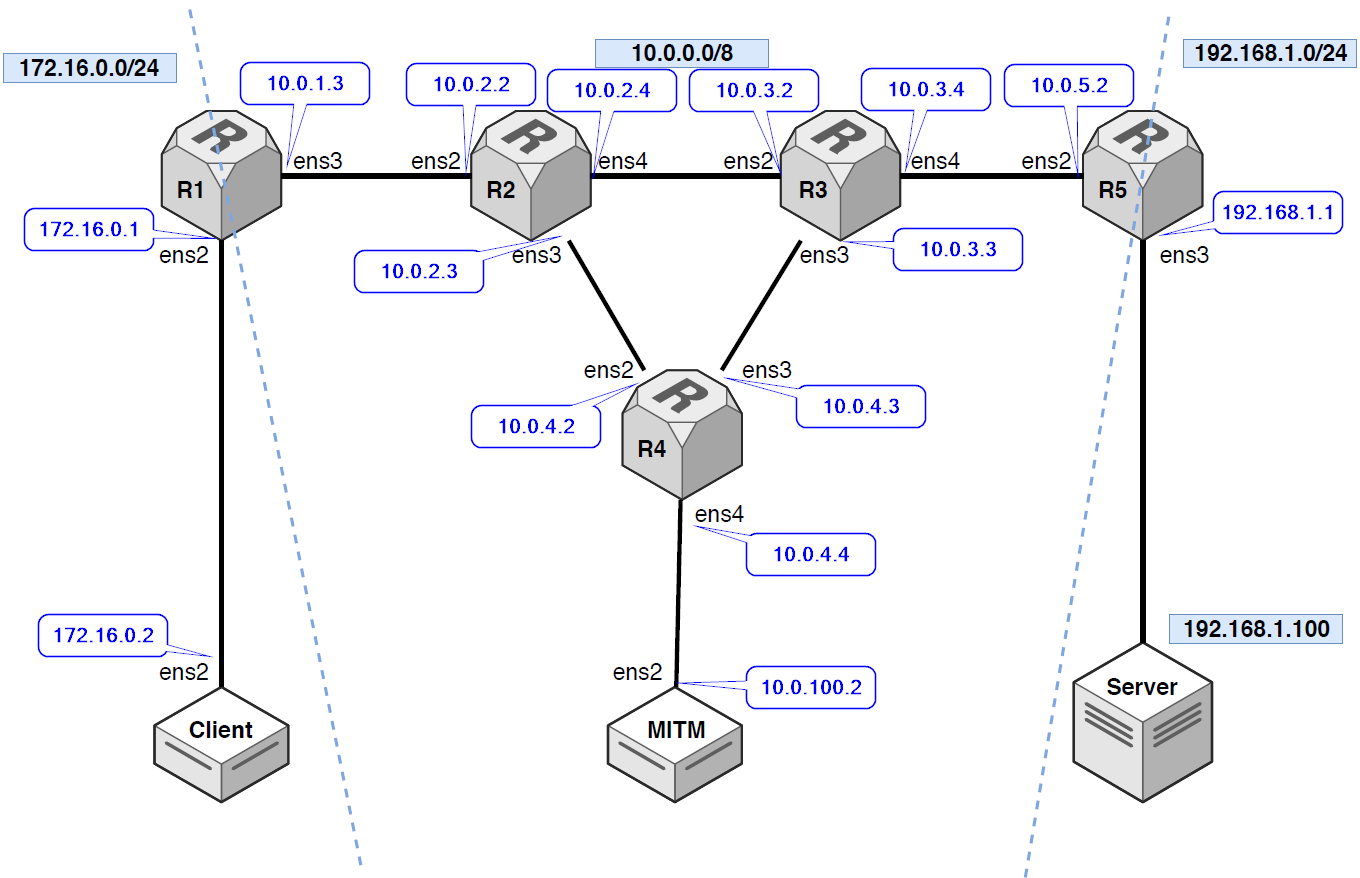
\includegraphics[width=0.90\textwidth]{images/netplan.png}
    \caption{Netplan}
    \label{fig:Netplan}
  \end{center}
\end{figure}

Wir ändern den netplan mit \lstinline{sudo nano /etc/netplan/50-cloud-init.yaml}.
\begin{lstlisting}
# This file is generated from information provided by
# the datasource.  Changes to it will not persist across an instance.
# To disable cloud-init's network configuration capabilities, write a file
# /etc/cloud/cloud.cfg.d/99-disable-network-config.cfg with the following:
# network: {config: disabled}
network:
    version: 2
    ethernets:
        ens2:
            dhcp4: false
            addresses: [172.16.0.1/24]
\end{lstlisting}

\subsection{BIRD}
\label{subsec:BIRD}
\begin{shadedquotation}
  Now, your routers must run OSPF. ...
  \begin{itemize}
    \item OSPFv2 must run on the routers.
    \item Find a way to protect the CPU from too much OSPF processing.
    \item A restart of BIRD should not result in lost routes.
  \end{itemize}
\end{shadedquotation}

\subsection{IP Forwarding}
\label{subsec:IPForwarding}

\par\medskip

\section{Verifizierung}
\label{sec:Verifizierung}
\begin{shadedquotation}
  Verify your routing implementation. Explain which exact commands you used for each verification step and show how they provide prove that your setup works.
\end{shadedquotation}

\subsection{Route Failover}
\label{subsec:RouteFailover}
\begin{shadedquotation}
  Verify that your setup works. Prove that a route failover takes place in case ofa route outage. To do that, a well known tool can be used.
\end{shadedquotation}

\subsection{Passive Interfaces}
\label{subsec:PassiveInterfaces}
\begin{shadedquotation}
  Show that no OSPF packets are sent into the client and server networks,too.\lstinline!tcpdump! and \lstinline!tshark! are good tools for that, sniff on the suspicious interfaces and filter for OSPFv2 packets. To be sure that your filter works, sniff on an interface where you expect OSPF-messages, too.
\end{shadedquotation}

\subsection{Access Website}
\label{subsec:AccessWebsite}
\begin{shadedquotation}
  Finally, you must be able to access the webpage from the webserver. You can use \lstinline!curl! or \lstinline!wget! for that. The webserver listens on port 8080.
\end{shadedquotation}

\section{Performanz}
\label{sec:Performanz}
\begin{shadedquotation}
  Provide the measurement before and after the appliance of the \lstinline!tc! commands.
  
  Provide the exact used \lstinline!tc! commands.
\end{shadedquotation}

\section{Referenzblatt}
\label{sec:Referenzblatt}
\begin{shadedquotation}
  We also expect you to hand in a reference sheet for all the net-work commands used in this lab. Just list every command and its function. This reference must not be longer than one page.
\end{shadedquotation}

\par\medskip 

\begin{tabular}{ |p{4cm}|p{10cm}|}
  \hline
  \textbf{Befehl} & \textbf{Funktion} \\
  \hline
  \lstinline!tc! & Keine Ahnung \\
  \hline
  \lstinline!tc! & Wubbel \\
  \hline
\end{tabular}

\section{Anhänge}
\label{sec:Anhänge}

\subsection{Routing}
\label{subsec:Routing}
\begin{shadedquotation}
  \begin{itemize}
    \item Your delivered report must include the new usernames and pass-words of the hosts.
    \item Your delivery must contain the created netplan files and an ad-dress plan.
    \item Attach the BIRD config files to your cookbook and explain how you achieve the minimal requirements.
    \item Verify your routing implementation. Explain which exact commands you used for each verification step and show how they provide prove that your setup works.
  \end{itemize}
\end{shadedquotation}
Erarbeitung der BIRD-config ist im \ref{subsec:BIRD} erläutert.
Verifikation der Routing unter \ref{sec:Verifizierung}.

\subsection{Firewall}
\label{subsec:Firewall}

\begin{shadedquotation}
  We’re interested in the used \lstinline!nmap! command, where the firewall runs and why you’ve choosen that location. Print the ruleset of the firewall and attach it to your report.
\end{shadedquotation}

\end{document}
